\section{Conceptual clarification}

\subsubsection{Big Data}

Big data can be defined as: larger, more complex data sets, that contains greater variety of data, arriving in increasing volumes and with more velocity. But these massive volumes of data can be used to address business problems you wouldn't have been able to tackle before. Therefore, in order to derive value from data, quality is a prerequisite for the analysis and use of big data.

\subsubsection{Data quality}
 Data quality is defined as the degree to which a set of characteristics inherent in the data meets stated expectations \cite{Iso8000}. Several dimensions are involved in defining quality. Each of these describes characteristics that can be measured or evaluated against specific expectations \cite{dama}.
 \begin{enumerate}[parsep=0cm,itemsep=0cm]
     \item \textbf{completeness}: which measures the absence of missing values (null or empty strings, missing numerical data);
     \item \textbf{uniqueness}: this dimension allows the analysis of unique values and duplicated data;
     \item \textbf{timeliness}: describes the degree of freshness of the data for the task to be performed and is closely related to the notions of frequency, of data update and volatility (speed at which data becomes irrelevant);
     \item \textbf{validity}: data is considered valid if it conforms to the requirements of its definition: format (email, date), type (numeric, real), range (variation interval);
     \item \textbf{accuracy}: this dimension assesses the extent to which an information system correctly describes or approximates the real world it is intended to model;
     \item \textbf{consistency}: according to Batini and Scannapieco cited by Ehrlinger, Rusz and Wöß \cite{ehrlinger2019survey} , consistency captures the violation of semantic rules defined on data, where elements can be tuples of relational tables or records in a file.
 \end{enumerate}

\begin{figure}[H]
  \caption{Data quality dimensions}  \label{fig:dama_uk}
  \begin{center}
    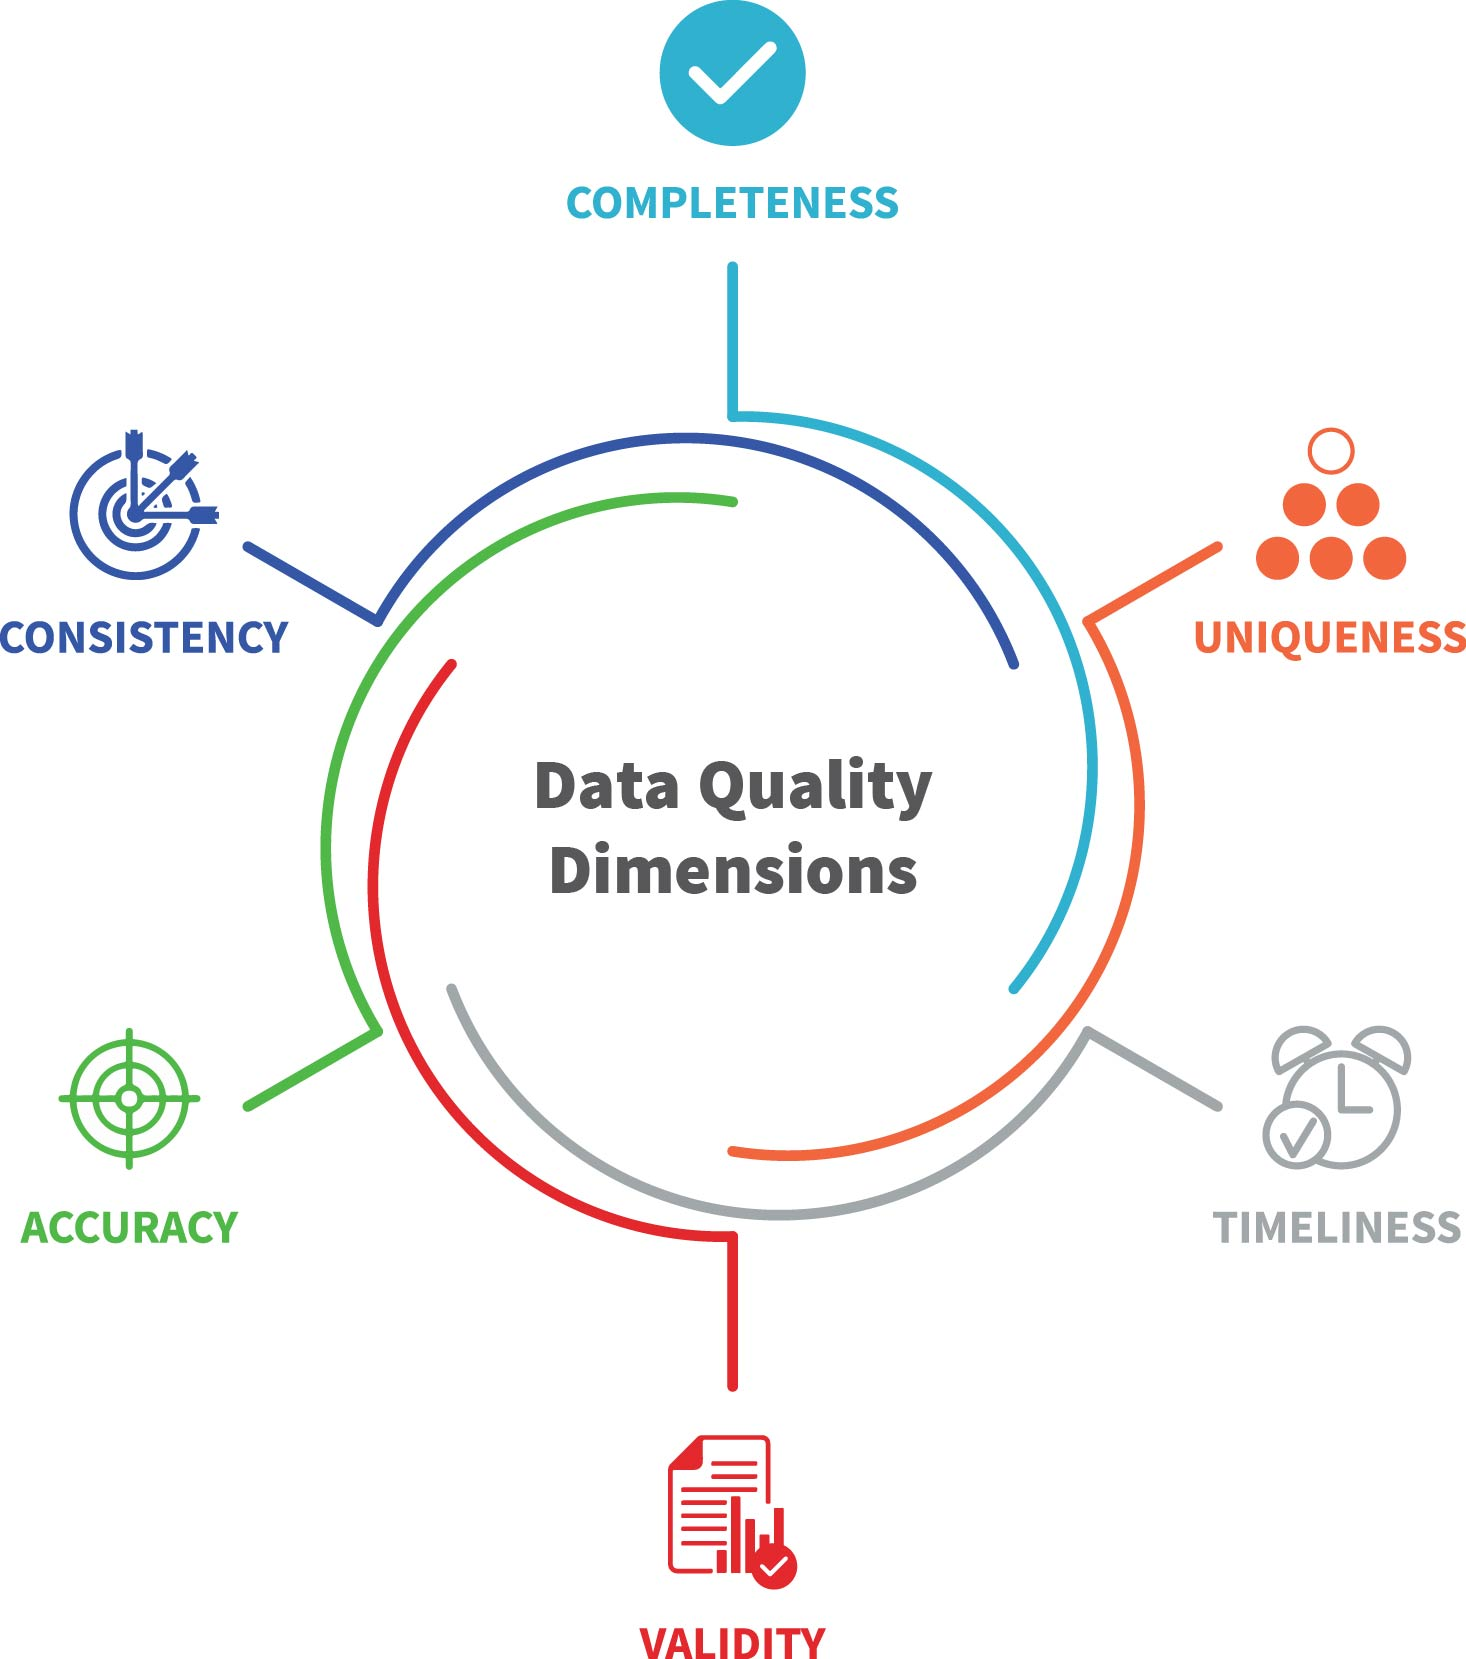
\includegraphics[scale=0.5]{Main/Static/data_quality_dimensions.jpg} 
  \end{center}
\end{figure}
To quantify each dimensions we use metrics. A data quality metric according to Ehrlinger, Rusz and Wöß \cite{ehrlinger2019survey}, is a function that associates a numerical value to a quality dimension. 